\pagestyle{fancy}

\fancyhf{}

\fancyhead[C]{Risultati}
\fancyfoot[C]{\thepage}

\fancypagestyle{plain}{
    \fancyhf{}
    \fancyfoot[C]{\thepage}
}

\chapter{Risultati}

\large

I risultati analizzati in questo capitolo fungono da solida base concettuale per orientare e alimentare riflessioni strategiche nell'ambito di potenziali sviluppi e progetti futuri correlati.

\bigskip

La presentazione dei risultati segue l'impiego completo di tutte le features illustrate nel capitolo 2, mostrando un quadro esaustivo delle dinamiche e delle metriche prodotte. Da sottolineare che il dataset fornito includeva già le features calcolate, rimuovendo così il processo dalla necessità di convertire il segnale dell'elettrocardiogramma in valori numerici.

\section{Preprocessing dei dati}

\begin{table}[t]
    \centering
    \begin{tabular}{|lrrrrcr|}
        \hline
        & \textbf{MEAN\_RR}
        & \textbf{MEDIAN\_RR}
        & \textbf{SDRR}
        & \textbf{RMSSD}
        & ...
        & \textbf{condition} \\
        \hline        
        count
        & 369289
        & 369289
        & 369289
        & 369289
        & ...
        & 369289 \\
        unique
        & NaN
        & NaN
        & NaN
        & NaN
        & ...
        & 3 \\
        top
        & NaN
        & NaN
        & NaN
        & NaN
        & ...
        & no stress \\
        freq
        & NaN
        & NaN
        & NaN
        & NaN
        & ...
        & 200082 \\
        mean
        & 846
        & 841
        & 109
        & 14
        & ...
        & NaN \\
        std
        & 124
        & 132
        & 77
        & 4
        & ...
        & NaN \\        
        min
        & 547
        & 517
        & 27
        & 5
        & ...
        & NaN \\        
        25\%
        & 760
        & 755
        & 64
        & 11
        & ...
        & NaN \\
        50\%
        & 822
        & 819
        & 82
        & 14
        & ...
        & NaN \\
        75\%
        & 924
        & 916
        & 118
        & 17
        & ...
        & NaN \\
        max
        & 1322
        & 1653
        & 563
        & 26
        & ...
        & NaN \\
        \hline
    \end{tabular}
    \caption{Riepilogo delle statistiche del dataset prima del preprocessing.}
    \label{tab:6-1}
\end{table}

Per cominciare, è stata studiata la struttura del dataset al fine di identificare le strategie di preprocessing da impiegare. In particolare, si è concentrata l'attenzione sul training set poiché è la parte di dataset utilizzata dalla macchina per apprendere e successivamente predire il testing set. Dopo una prima esecuzione, è stata eseguita un'analisi preliminare che ha permesso di ottenere un insieme di statistiche per ciascuna delle feature presenti, le quali sono riportate nella tabella \ref{tab:6-1}.

\bigskip

Grazie a questo riepilogo, è stata progettata l'implementazione del preprocessing secondo le seguenti considerazioni:

\begin{itemize}
    \item In base al riepilogo, sembra che non ci siano valori mancanti nelle features numeriche, poiché il conteggio per ogni feature è coerente.
    \item La label \texttt{condition} è una variabile categorica e ha tre valori unici. Questa feature deve essere codificata in un formato numerico adatto alla modellazione.
    \item La variabile \texttt{datasetId} ha un valore costante per tutte le osservazioni. Questa feature può essere eliminata perché non fornisce alcuna variabilità o informazione utile per l'analisi o la modellazione predittiva.
    \item Le features hanno intervalli e scale diverse, come si deduce dai valori minimi, massimi e dalle deviazioni standard. Questa differenza di scala può causare problemi con alcuni tipi di modelli. Si può prendere in considerazione la standardizzazione.
    \item L'ampia quantità di features potrebbe complicare la previsione del modello. Le tecniche di riduzione della dimensionalità, come la PCA, sono utilizzate per semplificare il dataset, riducendo il numero di variabili, mentre si cerca di mantenere il massimo delle informazioni rilevanti.
\end{itemize}

\bigskip

\begin{figure}[t]
    \begin{multicols}{2}
        \centering
        \includegraphics[width=\linewidth]{img//6/1.png}
        \caption{Matrice di correlazione con le features del dataset prima del preprocessing dei dati.}
        \label{fig:6-1}
        
        \columnbreak
        
        \includegraphics[width=\linewidth]{img//6/2.png}
        \caption{Diagramma a torta che mostra la percentuale di individui che hanno sperimentato ciascuna delle condizioni di stress durante l'esperimento.}
        \label{fig:6-2}
    \end{multicols}
\end{figure}

La figura \ref{fig:6-1}, presenta una matrice di correlazione costruita utilizzando le features del dataset prima del processo di preprocessing dei dati. La correlazione rappresenta la forza della relazione tra due variabili: una correlazione positiva indica un'associazione diretta tra le variabili, mentre una correlazione negativa indica un'associazione inversa tra le variabili.

\bigskip

La figura \ref{fig:6-2}, presenta un diagramma a torta che visualizza la percentuale di individui che hanno provato ciascuna delle condizioni di stress in questione durante l'esperimento.

\section{Classificazione}

\begin{figure}[t]
    \begin{multicols}{3}
        \centering
        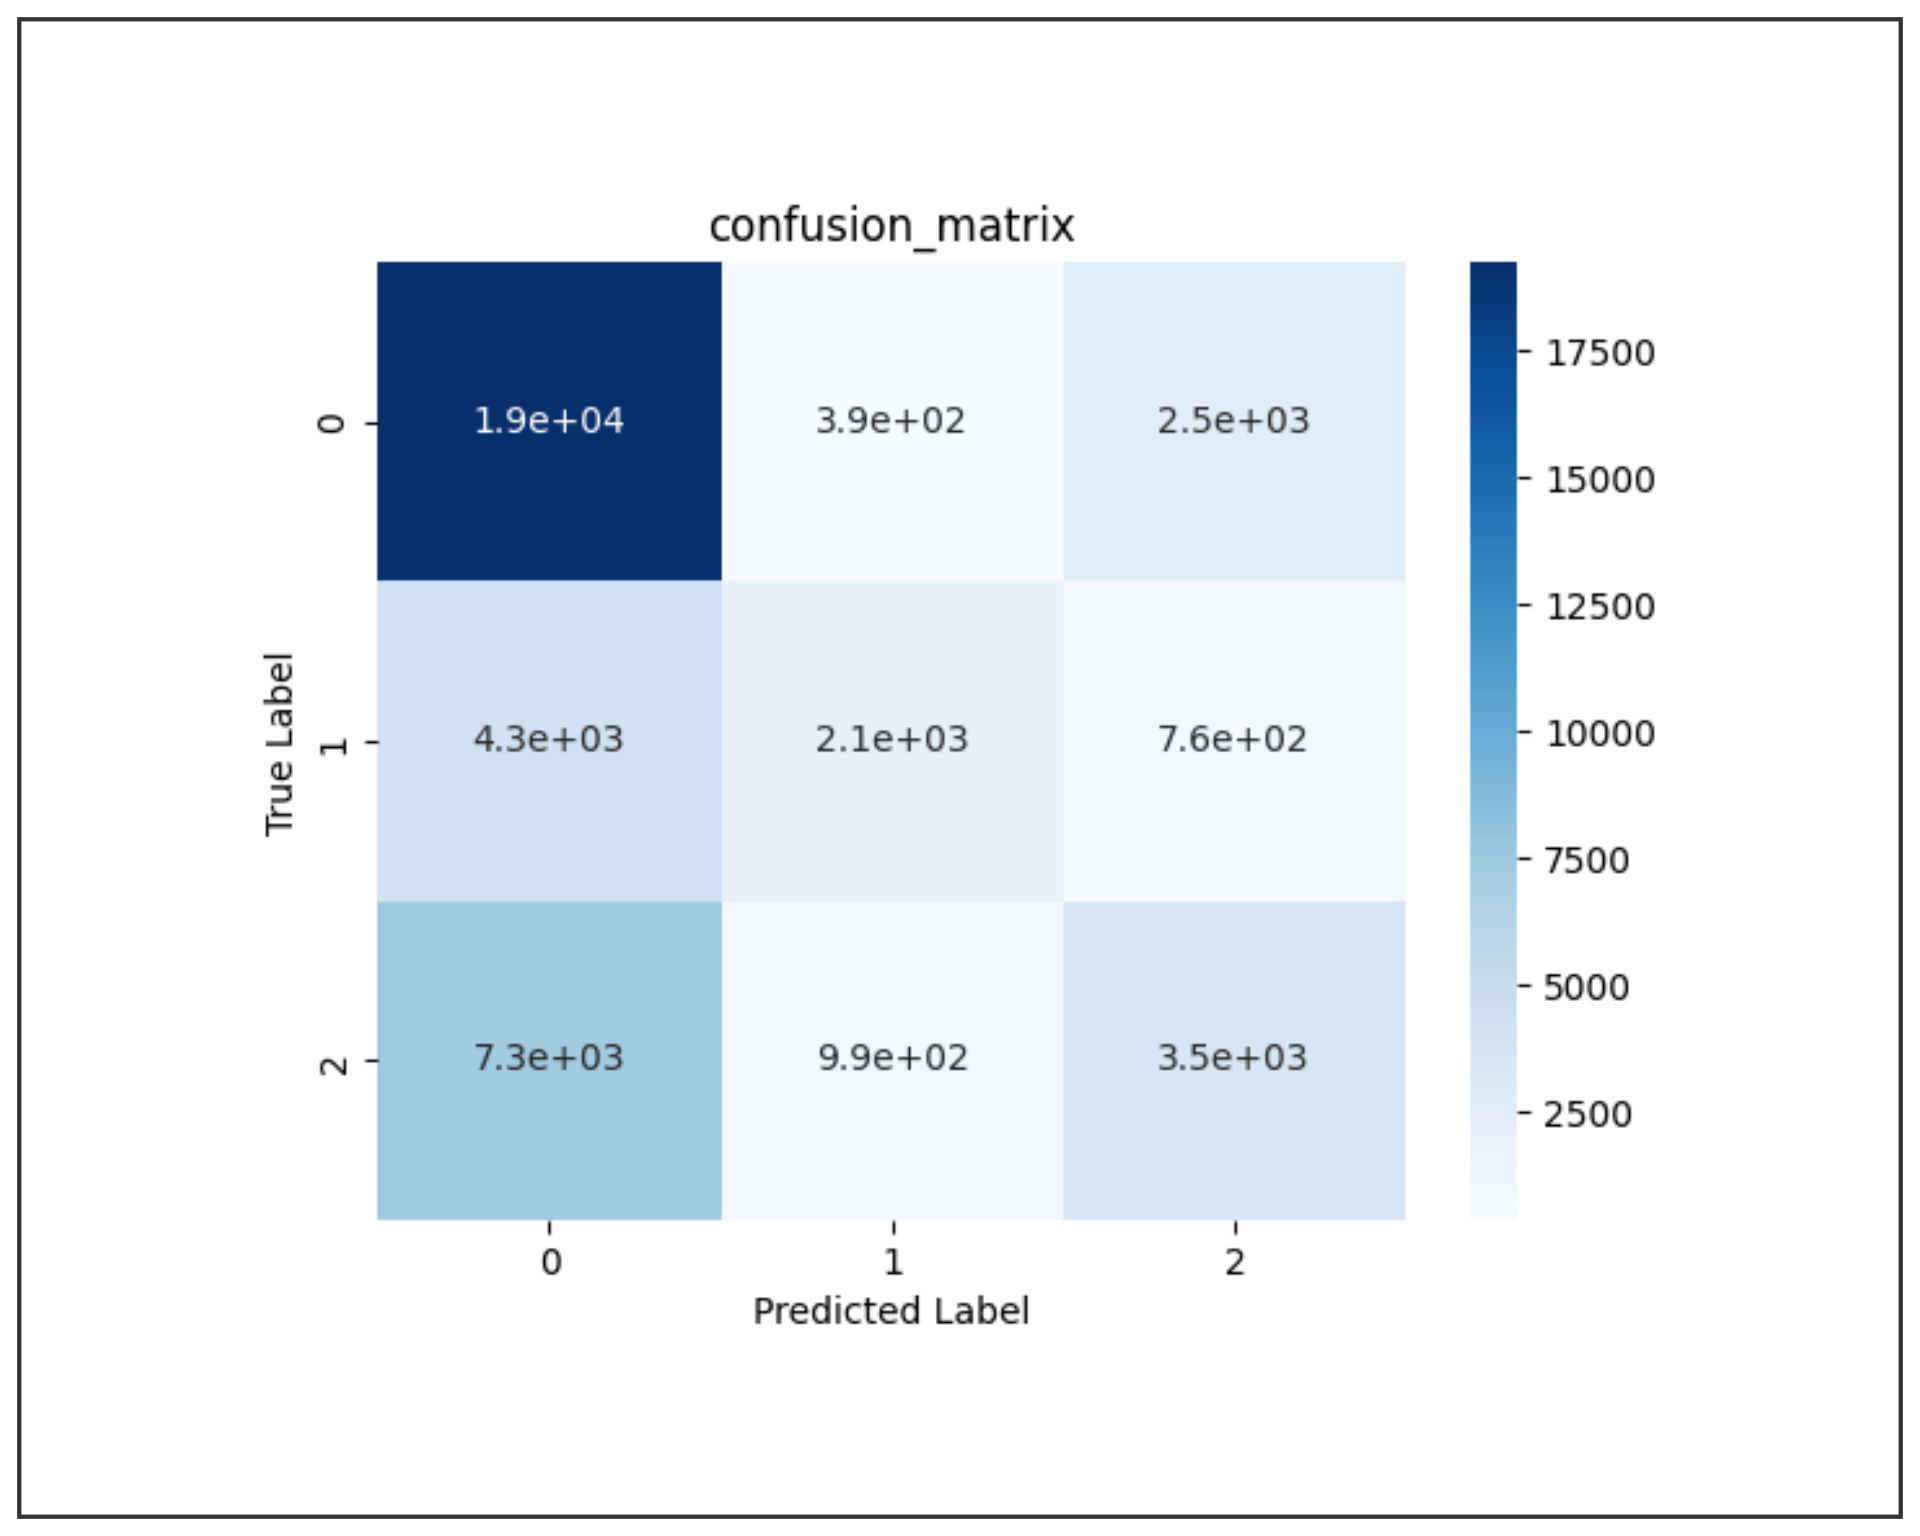
\includegraphics[width=\linewidth]{img//6/3.png}
        \caption{Matrice di confusione del logistic regression.}
        \label{fig:6-3}
        
        \columnbreak
        
        \includegraphics[width=\linewidth]{img//6/4.png}
        \caption{Matrice di confusione del decision tree.}
        \label{fig:6-4}

        \columnbreak
        
        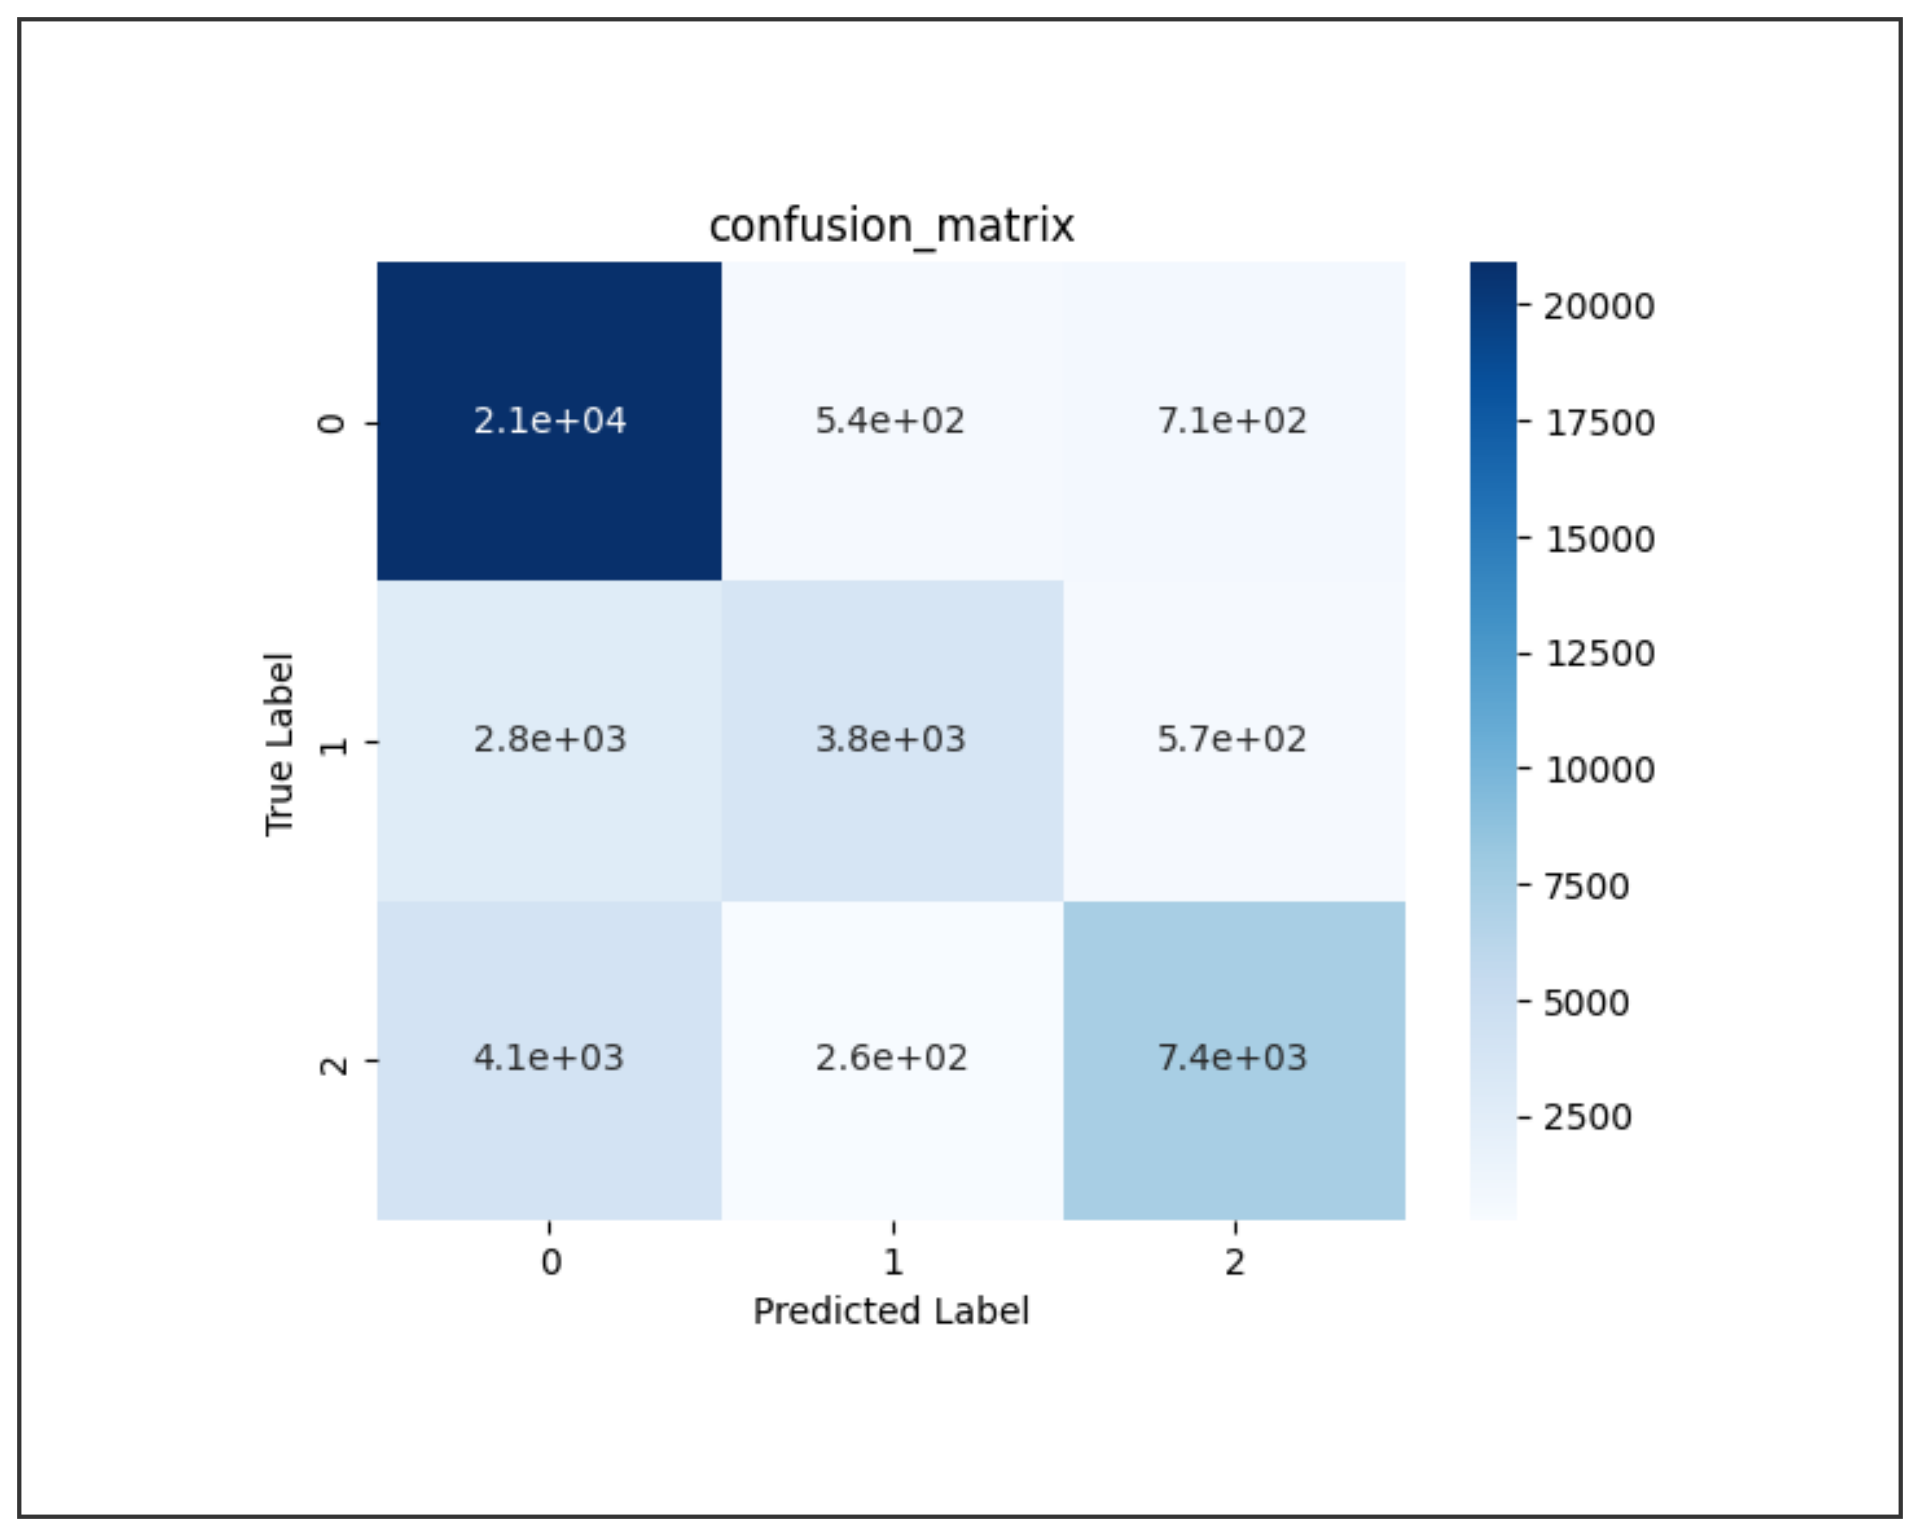
\includegraphics[width=\linewidth]{img//6/5.png}
        \caption{Matrice di confusione del random forest.}
        \label{fig:6-5}
    \end{multicols}
\end{figure}

Nel corso dell'apprendimento supervisionato, l'attenzione è stata concentrata esclusivamente sulla classificazione, con la valutazione di tre modelli: logistic regression, decision tree e random forest. L'obiettivo di questa scelta era esplorare le potenzialità e le prestazioni di ciascun modello, cercando di offrire una panoramica completa delle loro capacità e limitazioni nel problema correlato.

\subsection{Logistic regression}

\begin{table}[t]
    \centering
    \begin{tabular}{|r|rrrr|}
        \hline
        & \textbf{Precision}
        & \textbf{Recall}
        & \textbf{F1-score}
        & \textbf{Support} \\
        \hline
        \textbf{0}
        & 0.63
        & 0.87
        & 0.73
        & 22158 \\
        \textbf{1}
        & 0.60
        & 0.29
        & 0.39
        & 7093 \\
        \textbf{2}
        & 0.52
        & 0.30
        & 0.38
        & 11782 \\
        \textbf{Accuracy}
        &
        &
        & 0.61
        & 41033 \\
        \textbf{Macro Avg}
        & 0.58
        & 0.49
        & 0.50
        & 41033 \\
        \textbf{Weighted Avg}
        & 0.59
        & 0.61
        & 0.57
        & 41033 \\
        \hline
    \end{tabular}
    \caption{Risultati e metriche di performance del logistic regression.}
    \label{tab:6-2}
\end{table}

Come prima cosa, sono stati provati gli iperparametri adottati dagli autori del paper di riferimento \cite{iqbal2022exploring}. L'implementazione del modello è stata realizzata nel modo seguente:

\bigskip

\begin{lstlisting}
logistic_regression = LogisticRegression(
    solver='lbfgs',
    penalty='l2'
)
\end{lstlisting}

\bigskip

La tabella \ref{tab:6-2}, presenta i risultati e le metriche di performance ottenute a seguito di un'esecuzione del modello.

\bigskip

In conclusione, è stata realizzata una cross-validation su 10 fold, la media di questi valori, ha ottenuto un'accuratezza del 60.18\%.

\bigskip

Nella figura \ref{fig:6-3}, emerge dalla matrice di confusione che il modello mostra una buona capacità di predizione per la classe 0, con un numero significativo di predizioni corrette. Tuttavia, è evidente una certa confusione nella classe 1, dove il numero di falsi positivi è notevolmente superiore al numero di veri positivi. La classe 2 presenta una situazione simile, con un numero significativo di falsi positivi rispetto ai veri positivi.

\subsection{Decision tree}

\begin{table}[t]
    \centering
    \begin{tabular}{|r|rrrr|}
    \hline
    & \textbf{Precision}
    & \textbf{Recall}
    & \textbf{F1-Score}
    & \textbf{Support} \\
    \hline
    \textbf{0}
    & 0.64
    & 0.95
    & 0.76
    & 22158 \\
    \textbf{1}
    & 0.71
    & 0.37
    & 0.49
    & 7093 \\
    \textbf{2}
    & 0.80
    & 0.28
    & 0.42
    & 11782 \\
    \textbf{Accuracy}
    &
    &
    & 0.66
    & 41033 \\
    \textbf{Macro Avg}
    & 0.72
    & 0.53
    & 0.56
    & 41033 \\
    \textbf{Weighted Avg}
    & 0.70
    & 0.66
    & 0.62
    & 41033 \\
    \hline
    \end{tabular}
    \caption{Risultati e metriche di performance del decision tree.}
    \label{tab:6-3}
\end{table}

Inizialmente, sono stati ottimizzati gli iperparametri indicati dagli autori \cite{iqbal2022exploring}, poiché la vasta quantità di dati causava overfitting, portando il modello a una situazione di overtraining e generando prestazioni non realistiche. È stato necessario solo ridurre la profondità dell'apprendimento. L'implementazione pratica del modello è stata eseguita come segue:

\bigskip

\begin{lstlisting}
decision_tree = DecisionTreeClassifier(
    criterion='gini',
    max_depth=8,
    max_features='log2'
)
\end{lstlisting}

\bigskip

La tabella \ref{tab:6-3}, presenta i risultati e le metriche di performance generati in seguito all'esecuzione del modello.

\bigskip

In conclusione, è stata condotta una cross-validation su 10 fold, e la media di questi valori ha risultato in un'accuratezza del 74.47\%.

\bigskip

Nella figura \ref{fig:6-4}, si evidenzia dalla matrice di confusione che il modello mostra un'elevata precisione nella previsione della classe 0, con un numero significativo di predizioni corrette. Tuttavia, sono evidenti alcune aree di miglioramento, in particolare nelle classi 1 e 2. La classe 1 presenta un numero di falsi positivi otevolmente superiore al numero di veri positivi, indicando una certa confusione nella classificazione. Analogamente, nella classe 2, il numero di falsi positivi è sostanzialmente maggiore rispetto ai veri positivi.

\subsection{Random forest}

\begin{table}[t]
    \centering
    \begin{tabular}{|r|rrrr|}
        \hline
        & \textbf{Precision}
        & \textbf{Recall}
        & \textbf{F1-score}
        & \textbf{Support} \\
        \hline
        \textbf{0}
        & 0.74
        & 0.96
        & 0.83
        & 22158 \\
        \textbf{1}
        & 0.79
        & 0.51
        & 0.62
        & 7093 \\
        \textbf{2}
        & 0.89
        & 0.59
        & 0.71
        & 11782 \\
        \textbf{Accuracy}
        &
        &
        & 0.77
        & 41033 \\
        \textbf{Macro Avg}
        & 0.81
        & 0.68
        & 0.72
        & 41033 \\
        \textbf{Weighted Avg}
        & 0.79
        & 0.77
        & 0.76
        & 41033 \\
        \hline
    \end{tabular}
    \caption{Risultati e metriche di performance del random forest.}
    \label{tab:6-4}
\end{table}

Inizialmente, si è proceduto ottimizzando gli iperparametri raccomandati dagli autori \cite{iqbal2022exploring} al fine di affrontare il problema dell'overfitting, seguiti dalla stessa procedura adottata per il modello precedente. L'implementazione del modello è stata eseguita nel modo seguente:

\bigskip

\begin{lstlisting}
random_forest = RandomForestClassifier(
    criterion='gini',
    max_depth=8,
    max_features='log2',
    n_estimators=4
)
\end{lstlisting}

\bigskip

La tabella \ref{tab:6-4}, presenta i risultati e le metriche di performance ottenute dopo l'esecuzione del modello.

\bigskip

In conclusione, si è effettuata una cross-validation su 10 fold, e la media di tali valori ha prodotto un'accuratezza del 81.73\%.

\bigskip

Nella figura \ref{fig:6-5}, si deduce dalla matrice di confusione che il modello dimostra un'eccellente capacità di predizione nella classe 0, con un notevole numero di predizioni corrette. Tuttavia, sono presenti alcune aree di miglioramento nelle classi 1 e 2. Nella classe 1, il numero di falsi positivi supera considerevolmente il numero di veri positivi, indicando una certa confusione nella classificazione. Anche nella classe 2, il numero di falsi positivi è notevolmente superiore rispetto ai veri positivi.

\section{Clustering}

\begin{figure}[t]
    \begin{multicols}{3}
        \centering
        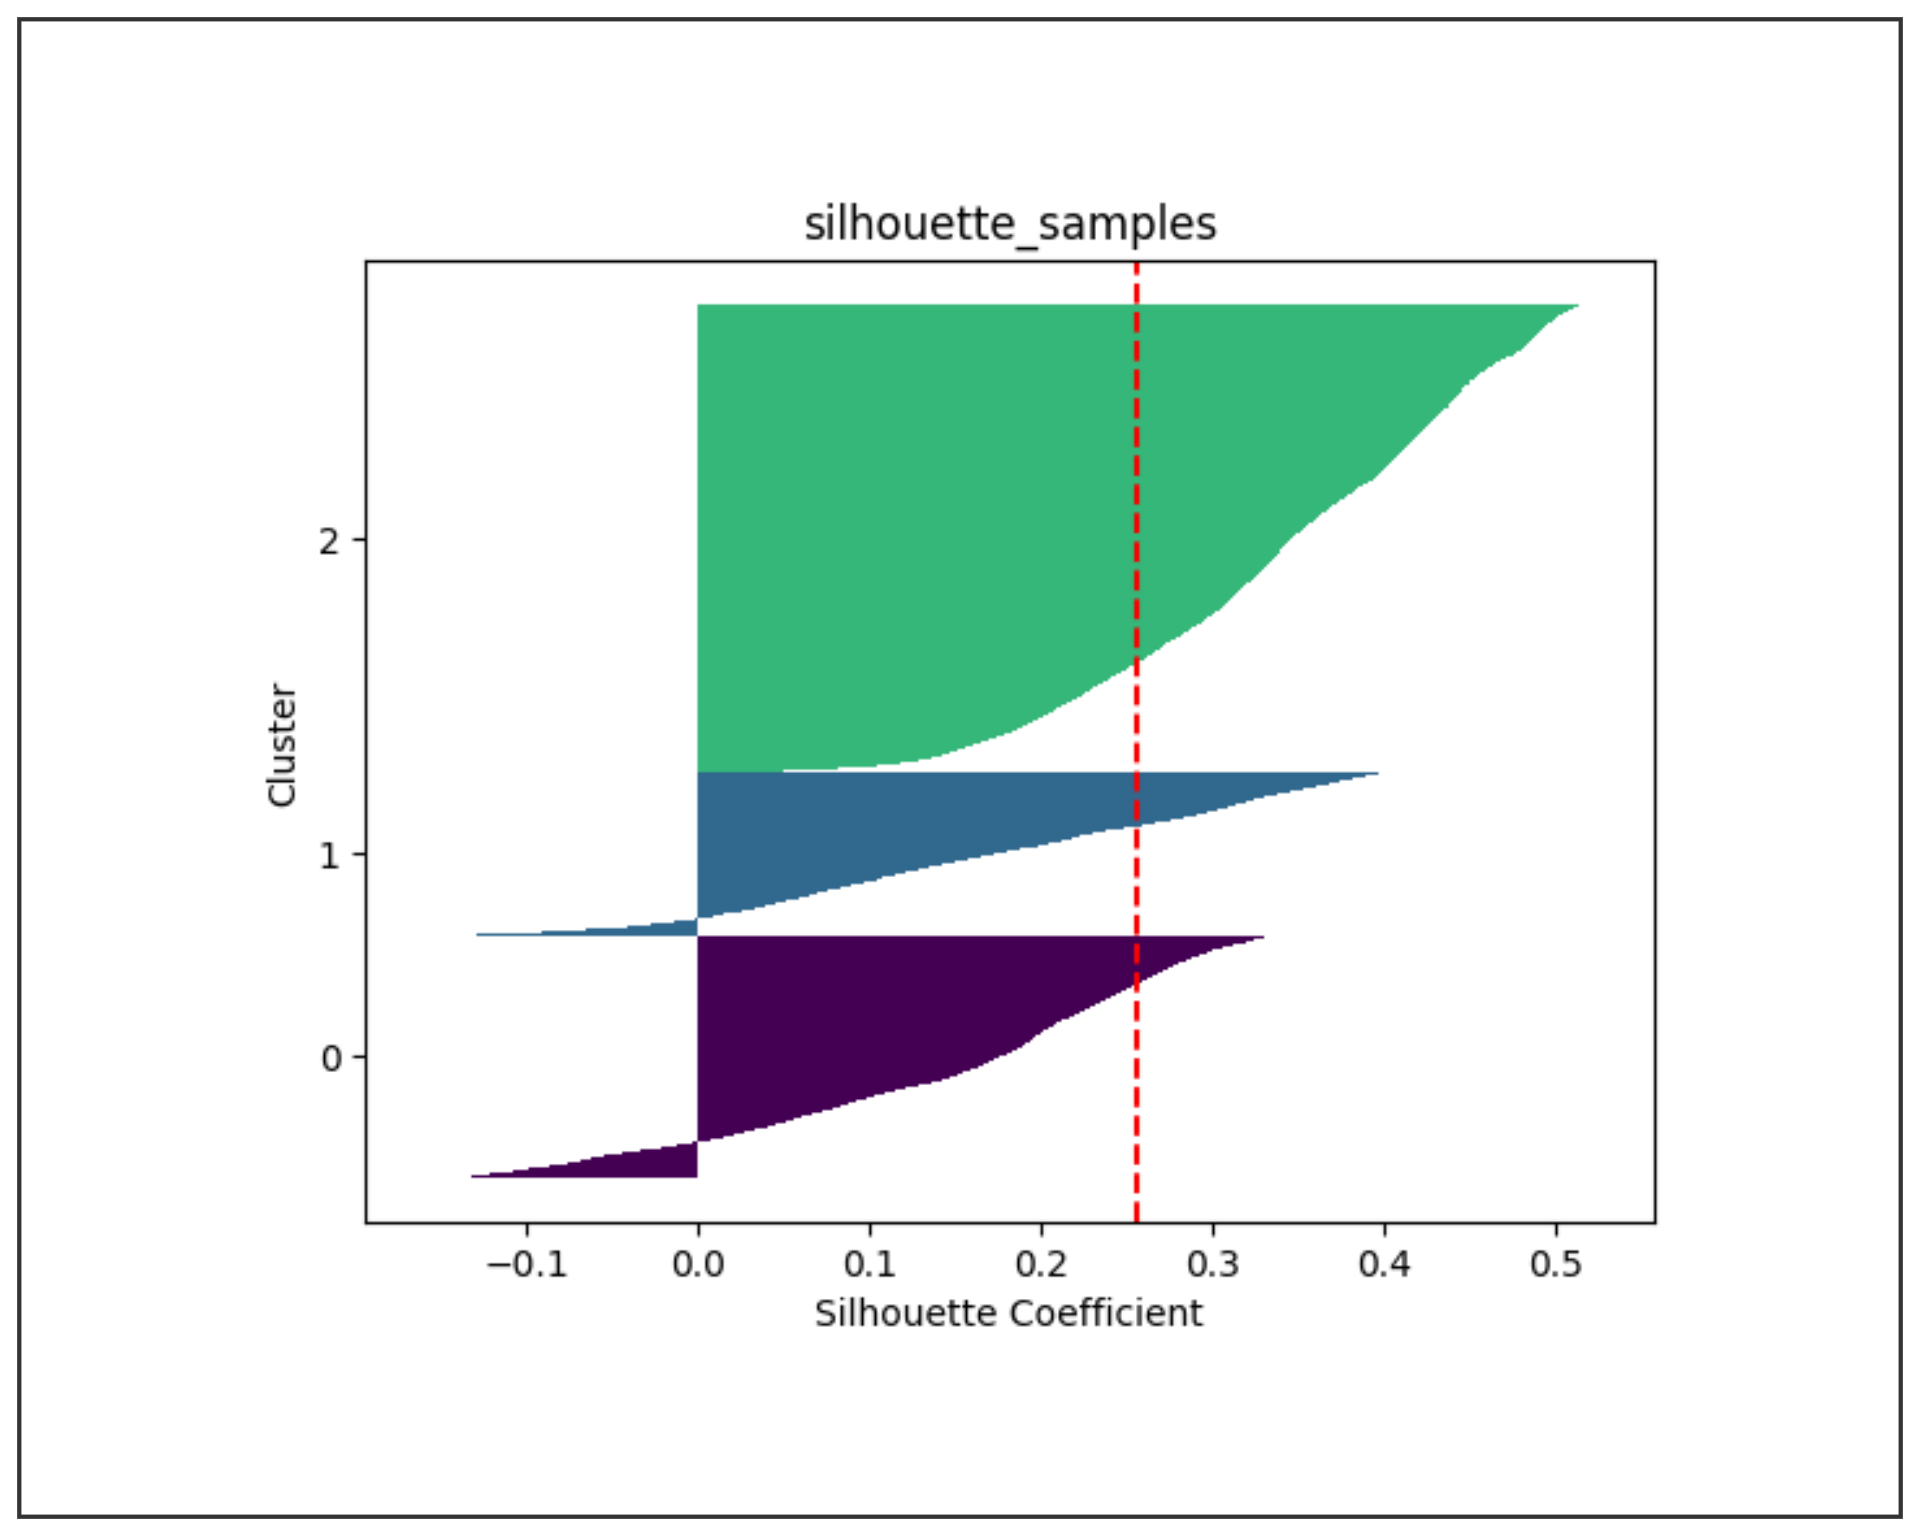
\includegraphics[width=\linewidth]{img//6/6.png}
        \caption{Grafico silhouette del k-means.}
        \label{fig:6-6}
        
        \columnbreak
        
        \includegraphics[width=\linewidth]{img//6/7.png}
        \caption{Grafico silhouette del gaussian mixture.}
        \label{fig:6-7}

        \columnbreak
        
        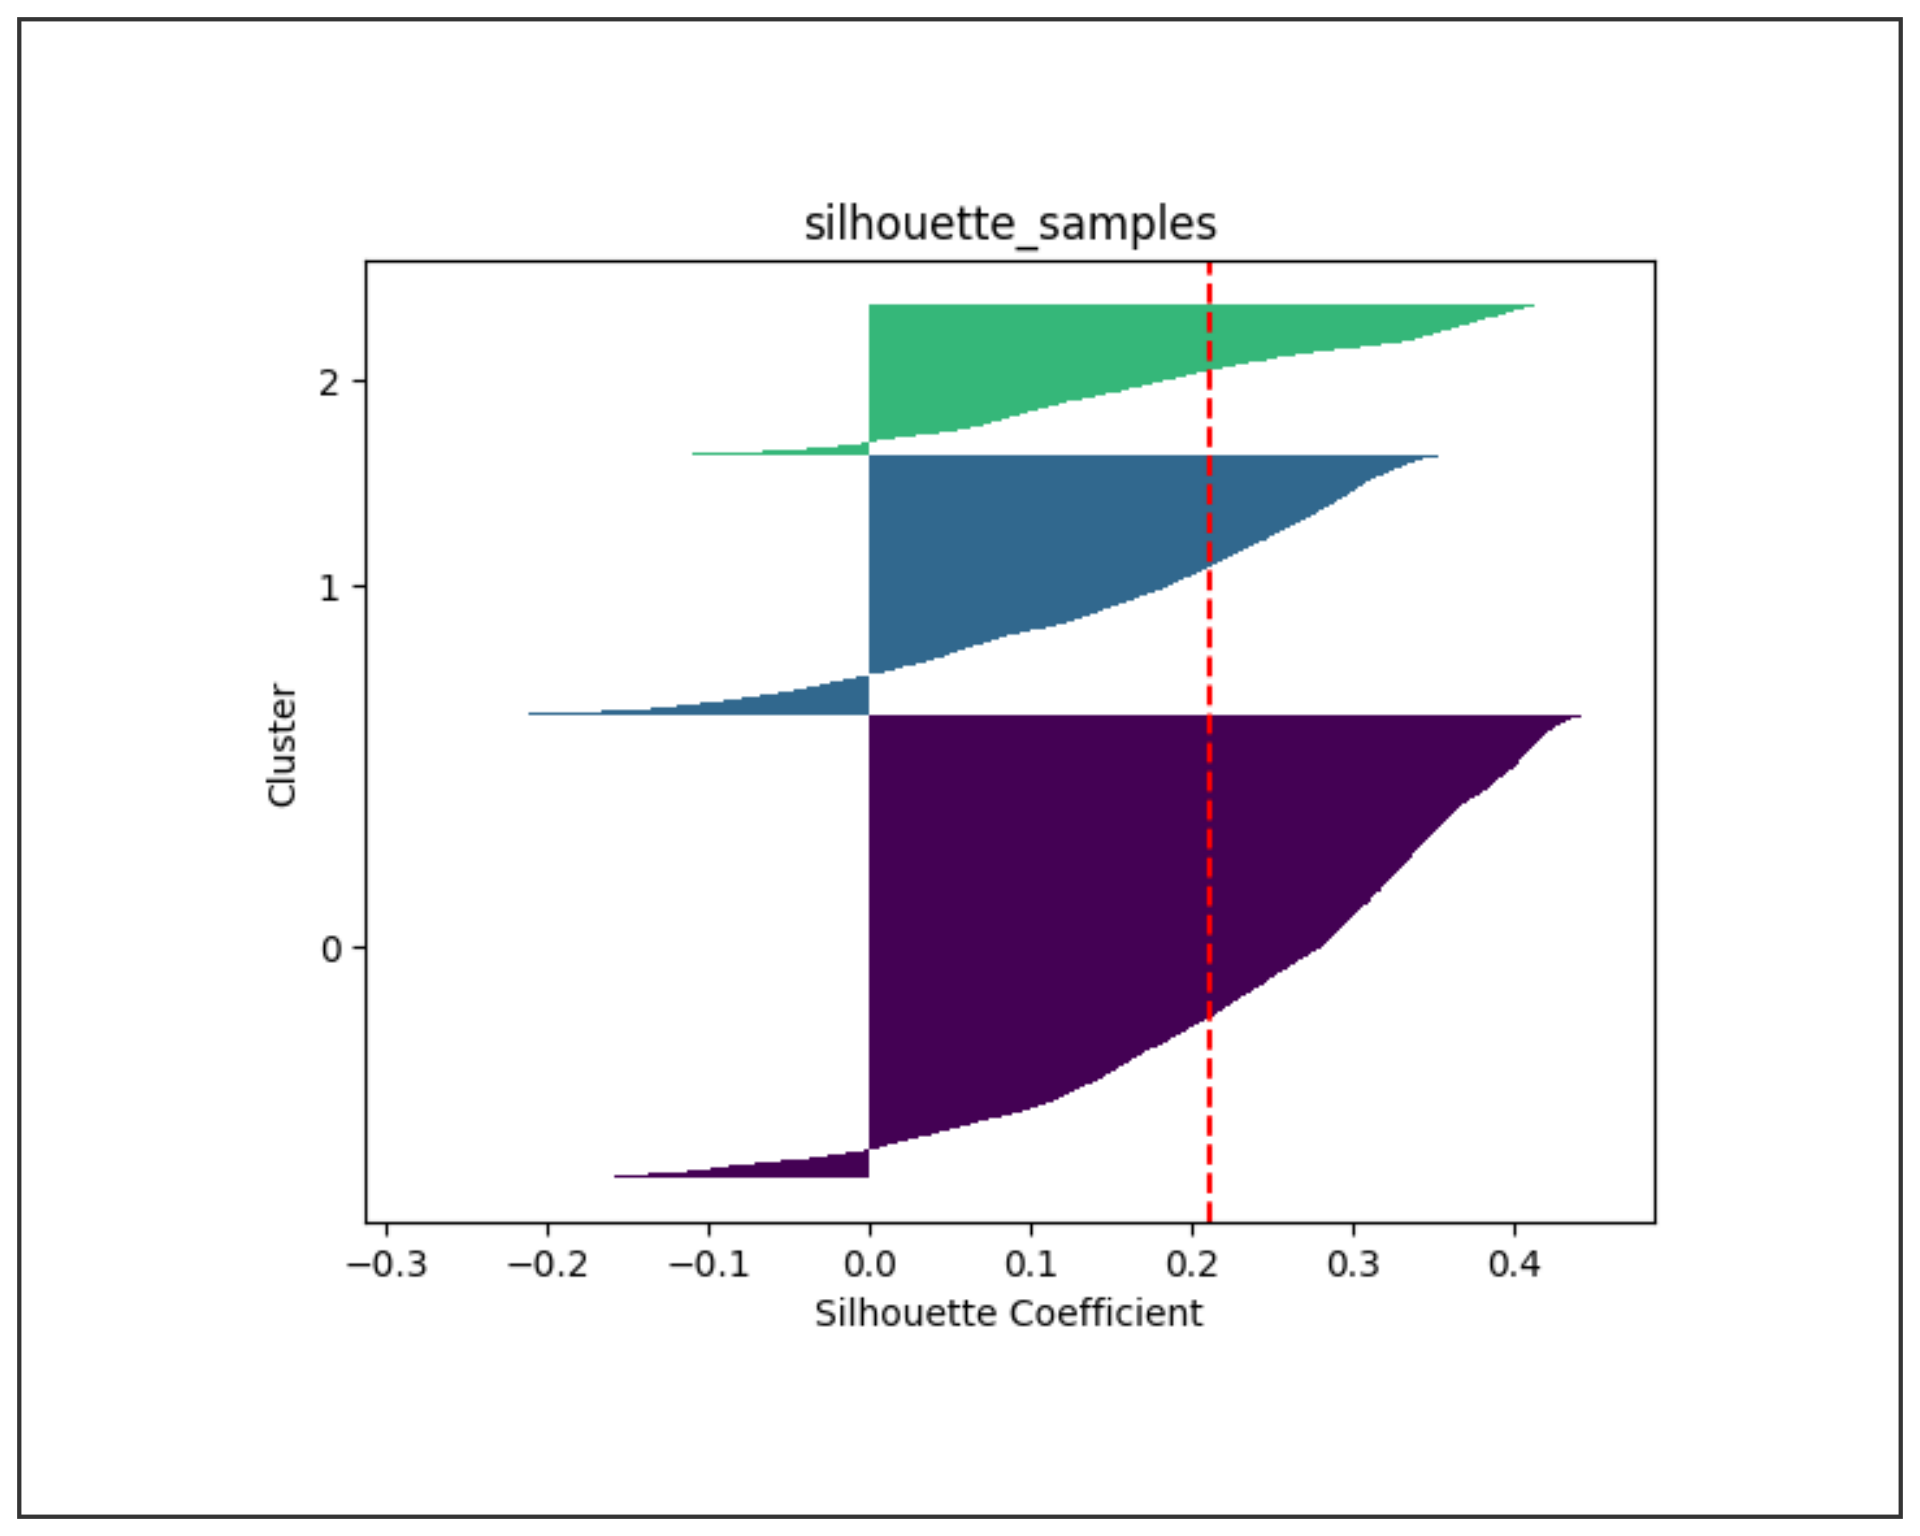
\includegraphics[width=\linewidth]{img//6/8.png}
        \caption{Grafico silhouette del BIRCH.}
        \label{fig:6-8}
    \end{multicols}
\end{figure}

Per l'apprendimento non supervisionato, il focus principale è stato sul clustering. Nello specifico, sono stati sperimentati tre modelli: k-means, gaussian mixture e BIRCH. Questa selezione è stata fatta per esplorare le potenzialità e le performance di ciascun modello, con lo scopo specifico di confrontare le prestazioni tra approcci supervisionati e non supervisionati.

\subsection{K-means}

Per cominciare, è stato fondamentale determinare il numero di cluster da utilizzare. Sebbene gli autori \cite{iqbal2022exploring} consigliassero l'impiego di due cluster, l'analisi ha dimostrato che con tre cluster le prestazioni miglioravano. Il modello è stato implementato nel modo seguente:

\bigskip

\begin{lstlisting}
kmeans = KMeans(n_clusters=3)
\end{lstlisting}

\bigskip

Il modello ha individuato un valore di punteggio silhouette pari a 0.2562, indicando così la coerenza e la distinzione efficace dei cluster nell'analisi.

\bigskip

Nella figura \ref{fig:6-6}, il coefficiente silhouette manifesta un valore medio di 0.2. Tale dato sottolinea la coerenza nelle definizioni e nelle distinzioni delle strutture dei dati oggetto dell'analisi.

\subsection{Gaussian mixture}

Inizialmente, è stato necessario determinare il numero di cluster; sebbene gli autori \cite{iqbal2022exploring} consigliassero l'uso di due cluster, l'adozione di tre ha portato a risultati migliori in termini di prestazioni. Di conseguenza, l'implementazione del modello è stata realizzata nel seguente modo:

\bigskip

\begin{lstlisting}
gaussian_mixture = GaussianMixture(n_components=3)
\end{lstlisting}

\bigskip

Il modello ha identificato un coefficiente di silhouette pari a 0.0928, evidenziando una moderata coerenza e distinzione tra i cluster nell'analisi effettuata. Questo valore suggerisce una separazione delle osservazioni, seppur con una certa sovrapposizione, indicando una struttura ragionevole ma potenzialmente migliorabile dei cluster identificati.

\bigskip

Nella figura \ref{fig:6-7}, il coefficiente silhouette manifesta un valore medio di 0.1. Tale dato sottolinea una misura di coerenza nelle definizioni delle strutture dei dati analizzati, anche se con una minore distinzione rispetto ad altre situazioni in cui il coefficiente silhouette potrebbe assumere valori più elevati.

\subsection{BIRCH}

Inizialmente, è stato necessario determinare il numero di cluster; sebbene gli autori \cite{iqbal2022exploring} consigliassero l'uso di due cluster, l'adozione di tre ha portato a risultati migliori in termini di prestazioni. Di conseguenza, l'implementazione del modello è stata realizzata nel seguente modo:

\bigskip

\begin{lstlisting}
birch = Birch(n_clusters=3)
\end{lstlisting}

\bigskip

Il modello ha rilevato un coefficiente di silhouette di 0.2117, suggerendo una coerenza significativa e una distinzione efficace dei cluster nell'ambito dell'analisi.

\bigskip

Nella figura \ref{fig:6-8}, il coefficiente silhouette rivela un valore medio di 0.2. Questo dato evidenzia la consistenza nelle definizioni e nelle distinzioni delle strutture dei dati sottoposti all'analisi.

\section{Risultati dei modelli}

\begin{table}[t]
    \centering
    \begin{tabular}{|llll|}
        \hline
        \textbf{Algoritmo}
        & \textbf{Modello}
        & \textbf{Metrica}
        & \textbf{Punteggio} \\
        \hline
        Supervised
        & Logistic regression
        & Accuracy
        & 60.18\% \\
        Supervised
        & Decision tree
        & Accuracy
        & 74.47\% \\
        Supervised
        & Random forest
        & Accuracy
        & 81.73\% \\
        Unsupervised
        & K-means
        & Silhouette
        & 0.2562 \\
        Unsupervised
        & Gaussian mixture
        & Silhouette
        & 0.0928 \\
        Unsupervised
        & BIRCH
        & Silhouette
        & 0.2117 \\
        \hline
    \end{tabular}
    \caption{Risultati e metriche di performance dei diversi modelli.}
    \label{tab:6-5}
\end{table}

Nella tabella \ref{tab:6-5}, vengono presentate le prestazioni dei vari modelli esaminati nel contesto dello studio. Tra i modelli di classificazione, il random forest mostra l'accuratezza più elevata, seguita dal decision tree e dal logistic regression. Per il clustering, i risultati indicano che sia il k-means che il BIRCH ottengono buone prestazioni, mentre il gaussian mixture mostra un punteggio silhouette molto più associato a zero.

\bigskip

In linea generale, i risultati evidenziano che per la classificazione sono efficaci sia il decision tree che il random forest, mentre per il clustering si distinguono per efficacia il k-means e il BIRCH. È interessante notare che le buone prestazioni sono comparabili tra i metodi supervisionati e quelli non supervisionati, suggerendo una parità di efficienza tra le due metodologie.

\bigskip

Attraverso il notebook disponibile su \href{https://www.kaggle.com/code/robertovicario/swell-kw-stress-detection}{\underline{Kaggle}}, è possibile esplorare in dettaglio tutti i risultati acquisiti, accompagnati dai codici associati. Questa piattaforma fornisce un'interfaccia diretta per visualizzare e analizzare in profondità i dati e le implementazioni sottostanti.